\documentclass[11pt,a4paper]{article}
\usepackage[a4paper,margin=1.6cm]{geometry}
\usepackage{iftex}
  \usepackage[T1]{fontenc}
\usepackage{lmodern}
  \usepackage[utf8]{inputenc}
  \usepackage[default]{lato}
\usepackage[dvipsnames,table]{xcolor}
\usepackage{graphicx}
\usepackage{tikz}
\usepackage[most]{tcolorbox}
\usepackage{array,tabularx,booktabs,longtable,multirow}
\usepackage{enumitem}
\usepackage{hyperref}
\usepackage{fancyhdr}
\usepackage{lastpage}
\usepackage{titlesec}
\usepackage{pgfplots}
\pgfplotsset{compat=1.18}
\usetikzlibrary{calc,positioning}
\hypersetup{colorlinks=true,urlcolor=MidnightBlue,linkcolor=MidnightBlue}
\pagestyle{fancy}
\fancyhf{}
\fancyfoot[L]{\textcolor{gray}{Modele LaTeX MVP - Rapport harmonise}}
\fancyfoot[R]{\textcolor{gray}{\thepage/\pageref{LastPage}}}
\renewcommand{\headrulewidth}{0pt}
\renewcommand{\footrulewidth}{0pt}
\setlength{\parindent}{0pt}
\setlength{\parskip}{0.45em}

% ---------- PALETTE ----------
\definecolor{PrimaryBlue}{HTML}{0C4A7A}
\definecolor{AccentOrange}{HTML}{F28C28}
\definecolor{SectorGreen}{HTML}{63A33C}
\definecolor{SectorBlue}{HTML}{1F77B4}
\definecolor{SectorOrange}{HTML}{F28C28}
\definecolor{SectorPurple}{HTML}{7A5EA8}
\definecolor{SoftGray}{HTML}{F4F6F8}
\definecolor{MidGray}{HTML}{D9E1E8}
\definecolor{DarkText}{HTML}{1E2A35}
\definecolor{MutedText}{HTML}{5B6770}
\definecolor{SoftGreen}{HTML}{EAF4E2}
\definecolor{SoftBlue}{HTML}{E8F1F8}
\definecolor{SoftOrange}{HTML}{FFF1E3}
\definecolor{SoftPurple}{HTML}{F1ECF8}

\color{DarkText}
\titleformat{\section}{\Large\bfseries\color{PrimaryBlue}}{}{0pt}{}
\titleformat{\subsection}{\normalsize\bfseries\color{PrimaryBlue}}{}{0pt}{}
\titlespacing*{\section}{0pt}{0.8em}{0.4em}
\titlespacing*{\subsection}{0pt}{0.5em}{0.25em}

% ---------- DYNAMIC VARIABLES TO INJECT ----------
% Replace the values below from your backend before compilation.
\def\OrgName{ {{ report_identity.organization_name | replace('&', '\\&') | replace('%', '\\%') | replace('_', '\\_') if report_identity.organization_name else 'N/A' }} }
\def\ReportTitle{[TITRE CANONIQUE]}
\def\ReportSubtitle{[SOUS TITRE]}
\def\ReportYear{ {{ report_identity.report_year if report_identity.report_year else 'N/A' }} }
\def\RegionName{ {{ report_identity.region_name | replace('&', '\\&') | replace('%', '\\%') | replace('_', '\\_') if report_identity.region_name else 'N/A' }} }
\def\GenerationDate{[DATE GENERATION]}
\def\CountriesCount{[NB PAYS]}
\def\PeopleAssistedTotal{ {{ global_kpis.people_assisted_total if global_kpis.people_assisted_total else 'N/A' }} }
\def\AdvocacyReports{ {{ global_kpis.advocacy_reports_count if global_kpis.advocacy_reports_count else 'N/A' }} }
\def\ExecutiveSummary{[RESUME EXECUTIF]}
\def\MethodNote{[NOTE METHODOLOGIQUE]}
\def\QualityNote{[NOTE QUALITE]}
\def\SourceDocs{[SOURCES PDF]}
\def\TopCountriesSummary{[SYNTHESE TOP PAYS]}
\def\ExtractionConfidence{[SCORE CONFIANCE]}

% ---------- REUSABLE COMPONENTS ----------
\newtcolorbox{kpicard}[3][]{
  enhanced,
  colback=#2,
  colframe=#2,
  boxrule=0pt,
  arc=3mm,
  left=4mm,right=4mm,top=4mm,bottom=4mm,
  width=#3,
  #1
}

{% raw %}
\newcommand{\KPIBox}[4]{%
\begin{kpicard}{#1}{#2}
  {\scriptsize\bfseries\textcolor{MutedText}{#3}}\\[0.35em]
  {\fontsize{22}{24}\selectfont\bfseries\textcolor{PrimaryBlue}{#4}}
\end{kpicard}}

\newcommand{\SectorMiniCard}[5]{%
\begin{tcolorbox}[
  enhanced,
  colback=#2,
  colframe=#2,
  boxrule=0pt,
  arc=3mm,
  left=4mm,right=4mm,top=3mm,bottom=3mm,
  title={\textcolor{PrimaryBlue}{\bfseries #1}},
  coltitle=PrimaryBlue,
  fonttitle=\normalsize,
]
{\Large\bfseries\textcolor{PrimaryBlue}{#3}}\\[-0.2em]
{\small\textcolor{MutedText}{personnes assistees}}\\[0.3em]
{\footnotesize #4}\\[0.3em]
{\scriptsize\textcolor{MutedText}{#5}}
\end{tcolorbox}}

\newcommand{\Pill}[2]{%
\tikz[baseline=(n.base)]\node[fill=#1,rounded corners=8pt,inner xsep=7pt,inner ysep=3pt] (n) {\scriptsize\bfseries\textcolor{PrimaryBlue}{#2}};}


{% endraw %}
\begin{document}

% =============================================
% PAGE 1 - COVER
% =============================================
\thispagestyle{empty}
\begin{tikzpicture}[remember picture,overlay]
\end{tikzpicture}

\vspace*{1.25cm}
{\color{white}\fontsize{12}{14}\selectfont\bfseries \OrgName}\par
\vspace{0.6cm}
{\color{white}\fontsize{26}{29}\selectfont\bfseries \ReportTitle}\par
\vspace{0.3cm}
{\color{white}\fontsize{13}{16}\selectfont \ReportSubtitle}\par
\vspace{0.55cm}
{\color{white}\large \RegionName\ --- \ReportYear}\par

\vfill

\noindent\begin{minipage}[t]{0.31\linewidth}
\KPIBox{SoftBlue}{\linewidth}{PAYS COUVERTS}{\CountriesCount}
\end{minipage}\hfill
\begin{minipage}[t]{0.31\linewidth}
\KPIBox{SoftOrange}{\linewidth}{PERSONNES ASSISTEES}{\PeopleAssistedTotal}
\end{minipage}\hfill
\begin{minipage}[t]{0.31\linewidth}
\KPIBox{SoftGreen}{\linewidth}{PLAIDOYER}{\AdvocacyReports}
\end{minipage}

\vfill

\begin{tcolorbox}[
  enhanced,
  colback=white,
  colframe=white,
  boxrule=0pt,
  arc=2.5mm,
  left=4mm,right=4mm,top=3mm,bottom=3mm
]
\textbf{Objet du MVP}\quad Ce document est un \textbf{brief harmonise premium genere automatiquement} a partir de plusieurs rapports PDF source. Il illustre le format editorial final : previsualisation PDF, telechargement PDF et tracabilite des donnees.
\end{tcolorbox}

\vspace{0.4cm}
{\small\textcolor{MutedText}{Genere le \GenerationDate\quad|\quad Sources : \SourceDocs}}
\newpage

% =============================================
% PAGE 2 - EXECUTIVE SUMMARY + GLOBAL KPIS
% =============================================
\section*{Resume executif}
\begin{tcolorbox}[
  enhanced,
  colback=SoftGray,
  colframe=MidGray,
  boxrule=0pt,
  arc=2.5mm,
  left=5mm,right=5mm,top=4mm,bottom=4mm
]
\ExecutiveSummary
\end{tcolorbox}

\vspace{0.3cm}
\begin{minipage}[t]{0.47\linewidth}
\subsection*{KPI globaux}
\begin{tabular}{@{}m{\linewidth}@{}}
\KPIBox{SoftBlue}{\linewidth}{TOTAL PERSONNES ASSISTEES}{\PeopleAssistedTotal}\\[0.35em]
\KPIBox{SoftOrange}{\linewidth}{RAPPORTS DE PLAIDOYER}{\AdvocacyReports}\\[0.35em]
\KPIBox{SoftGreen}{\linewidth}{COUVERTURE GEOGRAPHIQUE}{\CountriesCount\ pays}
\end{tabular}

\vspace{0.5em}
\subsection*{Notes de lecture}
\begin{itemize}[leftmargin=1.2em,itemsep=0.35em,topsep=0.25em]
  \item Les volumes sectoriels peuvent \textbf{se chevaucher}. Ils ne doivent pas etre additionnes sans verification metier.
  \item Les pourcentages pays peuvent etre \textbf{arrondis} dans les sources.
  \item Les elements visuels ou labels partiellement lisibles doivent etre conserves avec \textbf{validation humaine}. 
\end{itemize}
\end{minipage}
\hfill
\begin{minipage}[t]{0.49\linewidth}
\subsection*{Repartition sectorielle}
\begin{tcolorbox}[
  enhanced,
  colback=white,
  colframe=MidGray,
  boxrule=0.4pt,
  arc=2.5mm,
  left=3mm,right=5mm,top=3mm,bottom=3mm
]
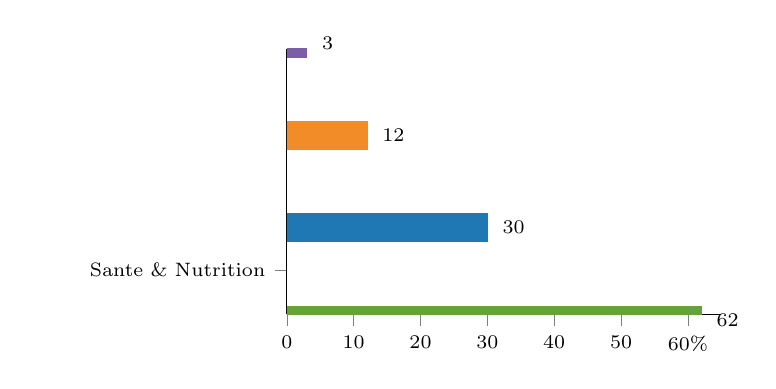
\begin{tikzpicture}
\begin{axis}[
  xbar,
  width=7.1cm,
  height=7.6cm,
  xmin=0,
  xmax=65,
  bar width=10pt,
  y=0.75cm,
  axis x line*=bottom,
  axis y line*=none,
  tick align=outside,
  xtick={0,10,20,30,40,50,60},
  xticklabels={0,10,20,30,40,50,60\%},
  symbolic y coords={Sante \& Nutrition,EHA / WASH,SAME / FSL,SMSP / MHPSS},
  ytick=data,
  yticklabel style={font=\scriptsize,text width=2.9cm,align=right},
  tick label style={font=\scriptsize},
  nodes near coords,
  every node near coord/.append style={font=\scriptsize, anchor=west, xshift=2pt},
  enlarge y limits=0.25,
]
\addplot[fill=SectorGreen,draw=SectorGreen] coordinates {(62,Sante \& Nutrition)};
\addplot[fill=SectorBlue,draw=SectorBlue] coordinates {(30,EHA / WASH)};
\addplot[fill=SectorOrange,draw=SectorOrange] coordinates {(12,SAME / FSL)};
\addplot[fill=SectorPurple,draw=SectorPurple] coordinates {(3,SMSP / MHPSS)};
\end{axis}
\end{tikzpicture}
\end{tcolorbox}

\vspace{0.3cm}
{\footnotesize\textcolor{MutedText}{Injecter ici les parts sectorielles standardisees et leurs libelles canoniques.}}
\end{minipage}
\newpage

% =============================================
% PAGE 3 - SECTOR RESULTS
% =============================================
\section*{Resultats sectoriels}
{\small\textcolor{MutedText}{Mise en page conseillee : quatre cartes sectorielles avec volume, sous-indicateurs cles et resume narratif.}}

\begin{tabular}{@{}m{0.485\linewidth}@{\hspace{0.02\linewidth}}m{0.485\linewidth}@{}}
\SectorMiniCard{% if sector_results|length > 0 %}{{ sector_results[0].sector_label_canonical | replace('&', '\\&') | replace('%', '\\%') | replace('_', '\\_') }}{% else %}N/A{% endif %}}{SoftGreen}{% if sector_results|length > 0 %}{{ sector_results[0].people_assisted if sector_results[0].people_assisted else "N/A" }}{% else %}N/A{% endif %}}{% if sector_results|length > 0 and sector_results[0].sub_indicators %}
{% for m in sector_results[0].sub_indicators[:4] %}
{{ m.metric_id | replace('_', '\\_') }}: {{ m.value if m.value else "N/A" }}{% if not loop.last %}\\newline {% endif %}
{% endfor %}
{% else %}N/A{% endif %}}{% if sector_results|length > 0 %}{{ sector_results[0].narrative_summary | replace('&', '\\&') | replace('%', '\\%') | replace('_', '\\_') if sector_results[0].narrative_summary else "No narrative summary extracted." }}{% else %}N/A{% endif %}} &
\SectorMiniCard{% if sector_results|length > 1 %}{{ sector_results[1].sector_label_canonical | replace('&', '\\&') | replace('%', '\\%') | replace('_', '\\_') }}{% else %}N/A{% endif %}}{SoftOrange}{% if sector_results|length > 1 %}{{ sector_results[1].people_assisted if sector_results[1].people_assisted else "N/A" }}{% else %}N/A{% endif %}}{% if sector_results|length > 0 and sector_results[0].sub_indicators %}
{% for m in sector_results[0].sub_indicators[:4] %}
{{ m.metric_id | replace('_', '\\_') }}: {{ m.value if m.value else "N/A" }}{% if not loop.last %}\\newline {% endif %}
{% endfor %}
{% else %}N/A{% endif %}}{% if sector_results|length > 0 %}{{ sector_results[0].narrative_summary | replace('&', '\\&') | replace('%', '\\%') | replace('_', '\\_') if sector_results[0].narrative_summary else "No narrative summary extracted." }}{% else %}N/A{% endif %}}\\[0.2cm]
\SectorMiniCard{% if sector_results|length > 2 %}{{ sector_results[2].sector_label_canonical | replace('&', '\\&') | replace('%', '\\%') | replace('_', '\\_') }}{% else %}N/A{% endif %}}{SoftBlue}{% if sector_results|length > 2 %}{{ sector_results[2].people_assisted if sector_results[2].people_assisted else "N/A" }}{% else %}N/A{% endif %}}{% if sector_results|length > 0 and sector_results[0].sub_indicators %}
{% for m in sector_results[0].sub_indicators[:4] %}
{{ m.metric_id | replace('_', '\\_') }}: {{ m.value if m.value else "N/A" }}{% if not loop.last %}\\newline {% endif %}
{% endfor %}
{% else %}N/A{% endif %}}{% if sector_results|length > 0 %}{{ sector_results[0].narrative_summary | replace('&', '\\&') | replace('%', '\\%') | replace('_', '\\_') if sector_results[0].narrative_summary else "No narrative summary extracted." }}{% else %}N/A{% endif %}} &
\SectorMiniCard{% if sector_results|length > 3 %}{{ sector_results[3].sector_label_canonical | replace('&', '\\&') | replace('%', '\\%') | replace('_', '\\_') }}{% else %}N/A{% endif %}}{SoftPurple}{% if sector_results|length > 3 %}{{ sector_results[3].people_assisted if sector_results[3].people_assisted else "N/A" }}{% else %}N/A{% endif %}}{% if sector_results|length > 0 and sector_results[0].sub_indicators %}
{% for m in sector_results[0].sub_indicators[:4] %}
{{ m.metric_id | replace('_', '\\_') }}: {{ m.value if m.value else "N/A" }}{% if not loop.last %}\\newline {% endif %}
{% endfor %}
{% else %}N/A{% endif %}}{% if sector_results|length > 0 %}{{ sector_results[0].narrative_summary | replace('&', '\\&') | replace('%', '\\%') | replace('_', '\\_') if sector_results[0].narrative_summary else "No narrative summary extracted." }}{% else %}N/A{% endif %}}
\end{tabular}

\vspace{0.35cm}
\begin{tcolorbox}[
  enhanced,
  colback=SoftGray,
  colframe=MidGray,
  boxrule=0pt,
  arc=2.5mm,
  left=5mm,right=5mm,top=4mm,bottom=4mm,
  title={\textcolor{PrimaryBlue}{\bfseries Logique de remplissage dynamique}},
  coltitle=PrimaryBlue,
  fonttitle=\normalsize
]
\begin{itemize}[leftmargin=1.2em,itemsep=0.35em,topsep=0.2em]
  \item \textbf{Secteur canonique} : Health \& Nutrition, WASH, Food Security \& Livelihoods, MHPSS \& Protection.
  \item \textbf{Sous-indicateurs} : injectes depuis le schema standard interne.
  \item \textbf{Resume narratif} : version harmonisee, courte, professionnelle, sans recopier integralement le rapport source.
  \item \textbf{Traite de coherence} : verifier que les sous-indicateurs et les unites restent interpretable par un lecteur metier.
\end{itemize}
\end{tcolorbox}
\newpage

% =============================================
% PAGE 4 - COUNTRY FOCUS
% =============================================
\section*{Focus pays}
\begin{minipage}[t]{0.62\linewidth}
\rowcolors{2}{SoftGray}{white}
\begin{tabularx}{\linewidth}{@{}>{\bfseries}l>{\raggedleft\arraybackslash}p{2.5cm}>{\raggedleft\arraybackslash}p{1.5cm}>{\raggedleft\arraybackslash}X@{}}
\rowcolor{PrimaryBlue!12}
Pays & Total assiste & Secteur dominant & Repartition sectorielle \\
{% for c in country_focus %}
{{ c.country_name_canonical | replace('&', '\\&') | replace('%', '\\%') }} &
{{ c.people_assisted if c.people_assisted else "N/A" }} &
{{ c.sector_shares_pct.get("health_nutrition", "N/A") }} &
{{ c.sector_shares_pct.get("health_nutrition", "N/A") }} / {{ c.sector_shares_pct.get("wash", "N/A") }} / {{ c.sector_shares_pct.get("food_security_livelihoods", "N/A") }} / {{ c.sector_shares_pct.get("mhpss_protection", "N/A") }} \\
{% endfor %}
\end{tabularx}
\end{minipage}
\hfill
\begin{minipage}[t]{0.34\linewidth}
\begin{tcolorbox}[
  enhanced,
  colback=SoftBlue,
  colframe=SoftBlue,
  boxrule=0pt,
  arc=2.5mm,
  left=4mm,right=4mm,top=4mm,bottom=4mm,
  title={\textcolor{PrimaryBlue}{\bfseries Lecture rapide}},
  coltitle=PrimaryBlue,
  fonttitle=\normalsize
]
\TopCountriesSummary
\end{tcolorbox}

\vspace{0.35cm}
\begin{tcolorbox}[
  enhanced,
  colback=SoftOrange,
  colframe=SoftOrange,
  boxrule=0pt,
  arc=2.5mm,
  left=4mm,right=4mm,top=4mm,bottom=4mm,
  title={\textcolor{PrimaryBlue}{\bfseries Variables a injecter}},
  coltitle=PrimaryBlue,
  fonttitle=\normalsize
]
\begin{itemize}[leftmargin=1.2em,itemsep=0.35em,topsep=0.2em]
  \item pays
  \item total personnes assistees
  \item parts sectorielles
  \item secteur dominant calcule
\end{itemize}
\end{tcolorbox}
\end{minipage}
\newpage

% =============================================
% PAGE 5 - METHOD, QUALITY, TRACEABILITY
% =============================================
\section*{Methodologie, qualite et tracabilite}
\begin{tcolorbox}[
  enhanced,
  colback=SoftGray,
  colframe=MidGray,
  boxrule=0pt,
  arc=2.5mm,
  left=5mm,right=5mm,top=4mm,bottom=4mm,
  title={\textcolor{PrimaryBlue}{\bfseries Note methodologique}},
  coltitle=PrimaryBlue,
  fonttitle=\normalsize
]
\MethodNote
\end{tcolorbox}

\vspace{0.3cm}
\noindent\begin{minipage}[t]{0.48\linewidth}
\begin{tcolorbox}[
  enhanced,
  colback=SoftGreen,
  colframe=SoftGreen,
  boxrule=0pt,
  arc=2.5mm,
  left=4mm,right=4mm,top=4mm,bottom=4mm,
  title={\textcolor{PrimaryBlue}{\bfseries Controle qualite}},
  coltitle=PrimaryBlue,
  fonttitle=\normalsize
]
\QualityNote
\vspace{0.5em}
\textbf{Score de confiance global :} \ExtractionConfidence
\end{tcolorbox}
\end{minipage}\hfill
\begin{minipage}[t]{0.48\linewidth}
\begin{tcolorbox}[
  enhanced,
  colback=SoftBlue,
  colframe=SoftBlue,
  boxrule=0pt,
  arc=2.5mm,
  left=4mm,right=4mm,top=4mm,bottom=4mm,
  title={\textcolor{PrimaryBlue}{\bfseries Provenance minimale}},
  coltitle=PrimaryBlue,
  fonttitle=\normalsize
]
\begin{itemize}[leftmargin=1.2em,itemsep=0.35em,topsep=0.2em]
  \item conserver les \textbf{pages source}
  \item conserver le \textbf{libelle source}
  \item conserver la \textbf{langue source}
  \item noter si extraction : \texttt{rule\_based}, \texttt{mapping}, ou \texttt{validation humaine}
\end{itemize}
\end{tcolorbox}
\end{minipage}

\vfill
\begin{center}
\textcolor{MutedText}{\small Ce template est concu pour une application qui : ingere des PDF, normalise les donnees, remplit un modele editorial LaTeX premium, compile le PDF et le propose en previsualisation puis en telechargement.}
\end{center}

\end{document}